% Created 2026-07-08 Wed 21:54
% Intended LaTeX compiler: pdflatex
\documentclass[presentation]{beamer}
\usepackage[utf8]{inputenc}
\usepackage[T1]{fontenc}
\usepackage{graphicx}
\usepackage{longtable}
\usepackage{wrapfig}
\usepackage{rotating}
\usepackage[normalem]{ulem}
\usepackage{amsmath}
\usepackage{amssymb}
\usepackage{capt-of}
\usepackage{hyperref}
\usetheme{Madrid}
\usecolortheme{}
\usefonttheme{}
\useinnertheme{}
\useoutertheme{}
\author{Danilo Sebastián Unapucha Unaucho $\backslash$\ Michael Sornoza $\backslash$\ Sebastián Arevalo}
\date{2026-07-04}
\title{Memoria Externa del Sistema}

\hypersetup{
 pdfauthor={Danilo Sebastián Unapucha Unaucho $\backslash$\ Michael Sornoza $\backslash$\ Sebastián Arevalo},
 pdftitle={Memoria Externa del Sistema},
 pdfkeywords={},
 pdfsubject={},
 pdfcreator={Emacs 29.3 (Org mode 9.6.15)}, 
 pdflang={Spanish}}
\begin{document}

\maketitle
\begin{frame}{Outline}
\tableofcontents
\end{frame}

\section{Discos de estado solido}
\label{sec:orga43b6c9}
\begin{frame}[label={sec:org048a9f3}]{Discos de estado solido}
Un disco de estado solido es formado a partir de componentes de estado
solido lo que significa que usan semiconductores de elementos solidos
como la silicona o galio. Estas memorias tienen chips basados en NANDS
\textbf{Ventajas del los discos de estado solido:}
\begin{itemize}
\item \textbf{Velocidad:} Tienen una velocidad de copiado generalmente de
200 a 550 Mbps bastante mas rapida que los 50 a 120 Mbps de los
discos duros.
\item \textbf{Uso de energia:} En promedio consumen 2-3 watts prologando
la duracion de la bateria.
\end{itemize}
\textbf{Desventajas de los discos de esado solido:}
\begin{itemize}
\item \textbf{Capacidad:} Normalmente tienen mas capacidad que los discos
duros en laptos pero en computadoras de escritorio los discos duros
ganan en este aspecto.
\item \textbf{Costo:} Aproximadamente custan \$0.17 por Gb que los discos
de estado solido.
\end{itemize}
\end{frame}
\section{Organización de un disco de estado solido}
\label{sec:org6e976e4}
\begin{frame}[label={sec:orgd7a331d},shrink=15]{Organización de un disco de estado solido}
\begin{columns}
\begin{column}{0.55\columnwidth}
\begin{itemize}
\item \textbf{Interface:} Es la parte que conecta de manera lógica el ssd
con el sistema host.
\item \textbf{Controller:} Provee ejecucion del firmware.
\item \textbf{Direccionador:} Provee la lógica de seleccionamiento de los
chips NANDS
\item \textbf{Cache:} Cache del sistema de memoria para tener mayor
velocidad.
\item \textbf{Correccion de errores:} Componente que se encarga de
detectar y corregir errores.
\item \textbf{Componentes de memoria flash:} Son los chips NANDS
encargados de guardar la información.
\end{itemize}
\end{column}
\begin{column}{0.45\columnwidth}
\begin{center}
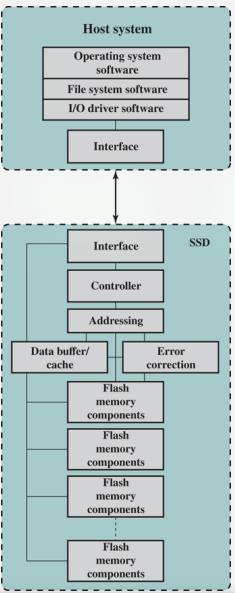
\includegraphics[width=0.8\linewidth]{images/organizacion_ssd.png}
\end{center}
\end{column}
\end{columns}
\end{frame}
\section{Problemas Prácticos}
\label{sec:org992f23c}
\begin{frame}[label={sec:orgfcd3a85},shrink=20]{Problemas Prácticos}
La naturaleza electrónica de las celdas Flash NAND introduce
restricciones físicas y operativas muy especificas en el hardware.

\textbf{Desafíos del medio semiconductor:}
\begin{itemize}
\item \textbf{ciclos P/E limitados:} Las celdas sufren un desgaste físico
\end{itemize}
irreversible en su capa aislante tras un numero fijo de escrituras o
borrados. 
\begin{itemize}
\item \textbf{Asimetría de bloques y paginas:} Las lecturas y escrituras
se ocurren a nivel de bloques completos.
\item \textbf{Wear Leveling:} Algoritmo integrado en el controlador para
distribuir de manera homogénea las escrituras en todo el medio y
evitar sectores muertos prematuros
\item \textbf{Gestión de bloques dañados:} Aislamiento lógico dinámico de
celdas fallidas para resguardar la integridad de los datos útiles.
\end{itemize}
\begin{block}{Ampliación de escritura}
Debido a la imposibilidad de sobrescribir datos en una pagina
directamente sin limpiar previamente todo su bloque contenedor, se
produce el fenómeno WAF (\textit{Write Amplification Factor}).

\begin{itemize}
\item \textit{Definición:} Ocurre cuando un controlador debe reubicar
dinámicamente paginas validas a un bloque limpio antes de borrar un
bloque viejo, generando escrituras internas añadidas.
\item \textit{Consecuencia:} Una alta amplificación satura los canales de
datos y acelera el fin de la vida útil del hardware. \\[0pt]
\end{itemize}

\vspace{0.3cm}
\hspace{3cm} \(waf + \frac{\text{Datos Escritos en la Memoria
Flash}}{\text{Datos Solicitados por el Host}}\)

\begin{definition}
El firmware busca aproximar el WAF los mas cercano posible a 1
mediante una recolección de basura optimizada en segundo plano.
\end{definition}
\end{block}
\end{frame}

\section{Memoria Óptica}
\label{sec:orge7672f2}
\begin{frame}[label={sec:org1621fec}]{Disco Compacto}
\begin{columns}
\begin{column}{0.6\columnwidth}
El almacenamiento óptico se basa en la reflexión de haces de luz
concentrados sobre una pista continua en espiral.
\begin{itemize}
\item \textbf{Pits (Hoyos):} Micro Hendiduras físicas estampadas en la
superficie de policarbonato que dispersan la luz del láser.
\item \textbf{Lands (Llanos):} Regiones intermedias altamente reflectantes
que devuelven el haz luminoso directamente al foto-diodo receptor.
\item \textbf{Codificación Binaria:} Las transiciones físicas entre un pit
y un land se interpretan como un bit '1', la continuidad se lee como
bits '0'.
\end{itemize}
\end{column}

\begin{column}{0.4\columnwidth}
\begin{center}
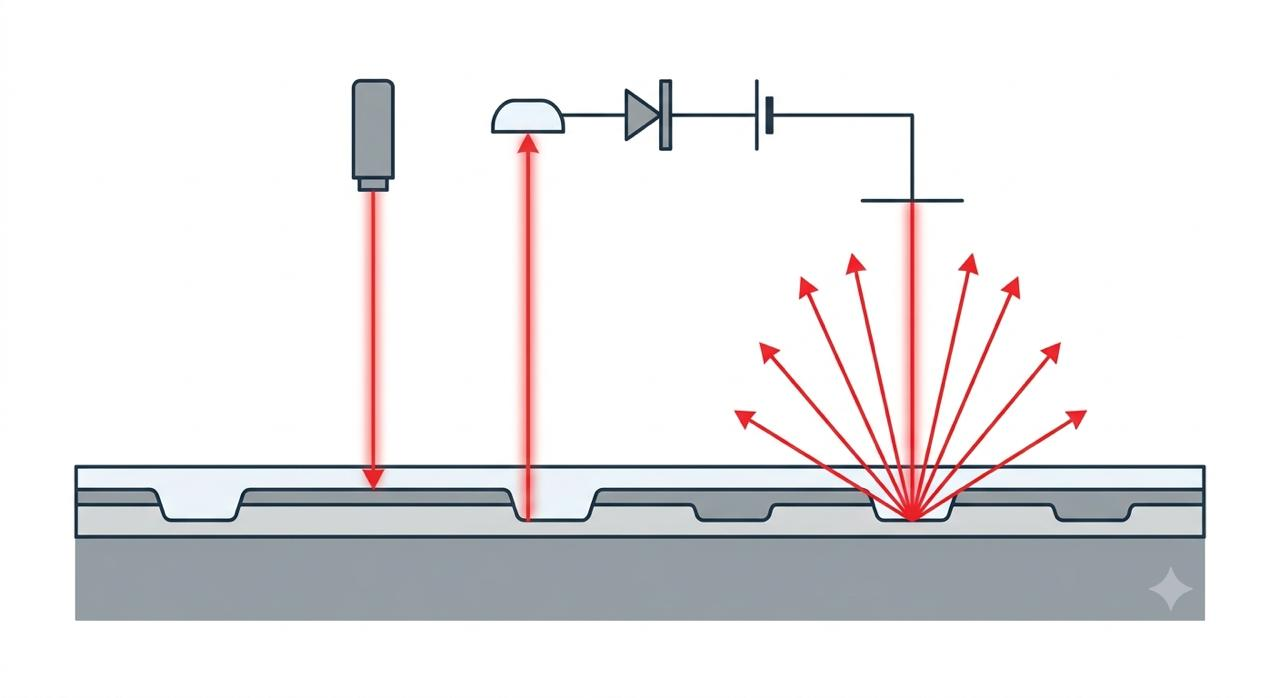
\includegraphics[width=1\linewidth]{images/Danilo_imgagen.jpeg}
\end{center}
\end{column}
\end{columns}
\end{frame}

\begin{frame}[label={sec:orgc512bc9}]{Variables del Formato CD}
La literatura de Stallings segmenta los discos compactos en tres
variaciones fundamentales según su capacidad de alternación 

\begin{itemize}
\item \textbf{CD-ROM:} Memoria de solo lectura cuyos pits y lands son
estampados en masa mediante molde de inyección de policarbonato industriales
\item \textbf{CD-R:} Disco grabable una única vez,  contiene una capa
intermedia de tinte orgánico translúcido que el láser quema a alta
potencia para emular opticamente un pit.
\item \textbf{CD-RW:} Medio regrabable estructurado con una aleación
metálica de fase capaz de alternar entre un estado cristalino
reflectante y amorfo absorbente.
\end{itemize}
\end{frame}

\section{DVD (Disco Digital  Versátil)}
\label{sec:orga03e559}

\begin{frame}[label={sec:orge85c416}]{Cambios en la llegada del DVD}
\begin{itemize}
\item Sustituto de las cintas VHS de video analógicas.
\item Sustituye a las cintas de video usadas en los reproductores de video (VCR).
\item Sustituye al CD-ROM en los PC y servidores.
\end{itemize}
\end{frame}

\begin{frame}[label={sec:org2ee30d6}]{Ventajas}
\begin{itemize}
\item Proporciona películas con una calidad de imagen impresionante, y se puede
acceder a ellos aleatoriamente como en los CD de audio, que también pueden leer los DVD.
\item En un disco se puede grabar un gran volumen de datos, en la actualidad siete veces más que en un CD-ROM
\item Los juegos para PC serán más reales y el software educativo incorporará más vídeo.
Como (habrá un nuevo pico en el tráfico en Internet e intranets corporativas, ya que este material se incorporará a los sitios web)
\end{itemize}
\end{frame}

\begin{frame}[label={sec:orge5ce178},shrink=15]{Capacidad del DVD}
\begin{itemize}
\item Los bits se empaquetan más juntos en un DVD. El espacio entre las vueltas de una espiral en un CD es de 1,6 µm y la distancia mínima entre hoyos a lo largo de la espiral es de 0,834 µm.
\item El DVD utiliza un láser con una longitud de onda menor y consigue un espaciado entre vueltas de 0,74 µm y una distancia mínima entre hoyos de 0,4 µm.
\item El resultado de estas dos mejoras supone un incremento de capacidad en un factor de siete, de alrededor de \textbf{4,7 GB}.
\item El DVD utiliza una segunda capa de hoyos y valles sobre la primera capa. Un DVD de doble capa tiene una capa semirreflectante sobre la capa reflectante, ajustando el enfoque, el láser puede leer cada capa por separado. Capacidad hasta \textbf{8,5 GB}.
\item El DVD-ROM puede tener dos superficies, mientras que en un CD los datos se graban solo en una superficie. Esto da una capacidad total de más de \textbf{17 GB}.
\end{itemize}

\begin{center}
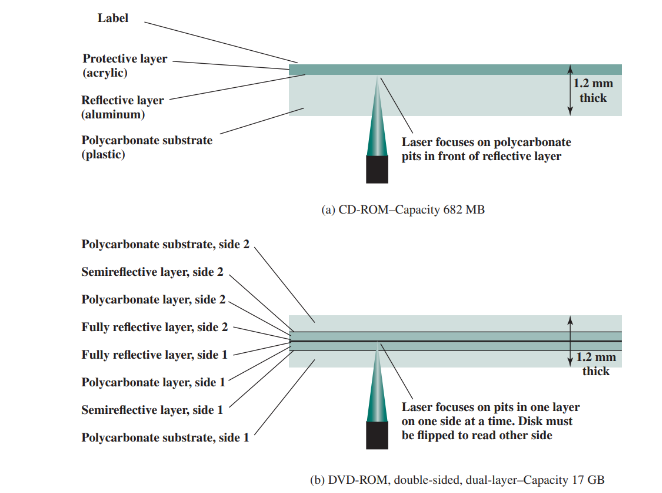
\includegraphics[width=0.45\linewidth]{images/DVD.png}
\end{center}
\end{frame}

\section{Discos Ópticos de Alta Definición}
\label{sec:org3942344}
\begin{frame}[label={sec:org6babeb7}]{Características}
\begin{itemize}
\item Diseñados para vídeo de alta definición y mayor capacidad que el DVD.
\item Usan láser de longitud de onda corta (azul-violeta) para mayor densidad de bits.
\item Dos formatos compitieron: \textbf{HD DVD} y \textbf{Blu-ray}.
\end{itemize}
\end{frame}

\begin{frame}[label={sec:orgffa2296},shrink=15]{Blue-ray}
\begin{itemize}
\item Logró la dominancia del mercado.
\item Capa de datos más cerca del láser: pistas e impresiones más pequeñas.
\item Capacidad de \textbf{25 GB} por capa.
\item Tres versiones: \textbf{BD-ROM} (solo lectura), \textbf{BD-R} (grabable una vez), \textbf{BD-RE} (regrabable).
\end{itemize}

\begin{center}
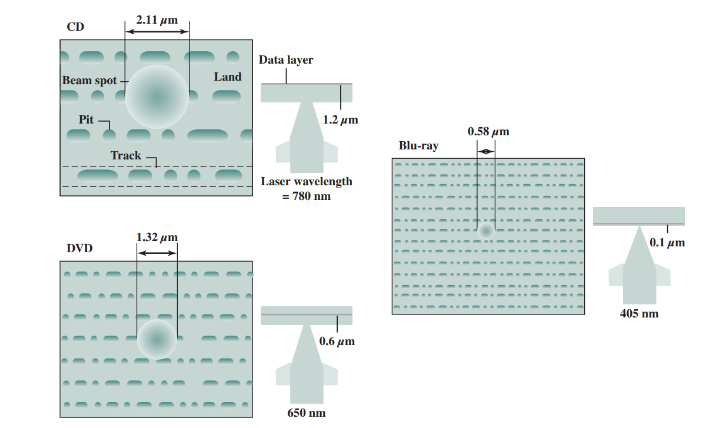
\includegraphics[width=0.55\linewidth]{images/AltaDefinicion.png}
\end{center}
\end{frame}
\end{document}
